\documentclass{article}
\usepackage[utf8]{inputenc}
\usepackage{hyperref}
\usepackage{tikz}
\usetikzlibrary{arrows.meta,positioning,shapes.geometric,fit}
\usepackage[backend=biber,style=numeric,sorting=none,sortcites,backref,natbib,hyperref]{biblatex}
\addbibresource{references.bib}

\title{Design Document - Recommender System for Research Papers \newline\newline \small Group 17}
\author{
  Matthias Bergmann (matr. nr.) \and
    Maximilian Herczegh (matr. nr.) \and
    Alexander Scheucher (matr. nr.) \and
    Patrick Ziegler (12303709)
}
\date{\today}

\begin{document}

\maketitle

\begin{abstract}
  With the evergrowing amount of research papers being published, it becomes increasingly difficult for researchers to
  stay updated in their respective fields and discover relevant literature. Especially finding the original sources and
  base materials for a specific topic can be a tedious task. To address this challenge, we propose the development and
  evaluation of a recommender system specifically designed to suggest relevant research papers based on short user
  queries. This differs from most existing research paper recommender systems, which expect an existing paper as the
  query. Due to the difficulty of user studies and live evaluations, we will focus on offline evaluation methods and how
  to use the citation graph for fine tuning and evaluation. Furthermore, we will compare different models
  and fine tuning methods to minimize the training effort in relation to achieved performance.
\end{abstract}

\section{Members and Roles}
\begin{itemize}
  \item Matthias Bergmann: ---
  \item Maximilian Herczegh: ---
  \item Alexander Scheucher: ---
  \item Patrick Ziegler: Dataset research, Data organization and preprocessing
\end{itemize}

\section{Dataset}
We will utilize the Semantic Scholar dataset collection accessible via thier API \cite{lo-wang-2020-s2orc}. This
includes more than 225 million papers, 100 million authors including paper-authorship data and a citation graph with
around 2.8 billion edges. Additionally, there exist pretrained embeddings we can compare to aswell as "tl;dr"
representations of the papers, usable as queries in during the recommender system evaluation. Furthermore, the API
provides a recommender system based on the graph and embedding information. However, this existing system is only built
to recommend new papers based on existing papers. We will utilize this information and evaluate the performance of
recommending papers soley based on short paragraphs and textual description as queries.

  {\color{red}TODO rethink below based on given recommender}
We will preprocess our data by generating the citation graph from the dataset and computing a similarity measure between each node in the graph. For this purpose we will experiment with different metrics or a combination, specifically bibliographic coupling, co-citation and personalized page rank.
Training samples will be generated from the dataset as follows. The input for our model will consist of two parts. First, a query which will be a small section of a paper from the datset. Second a different full paper from the dataset. The target variable will be the computed similarity score of the two papers.

\section{Evaluation and Metrics}
TODO explain how to use existing recommender

\section{Models and Comparison}

\section{Training and Fine-Tuning}

\newpage

% TODO: replace -> is currently just AI slop
\begin{figure}[h!]
  \centering
  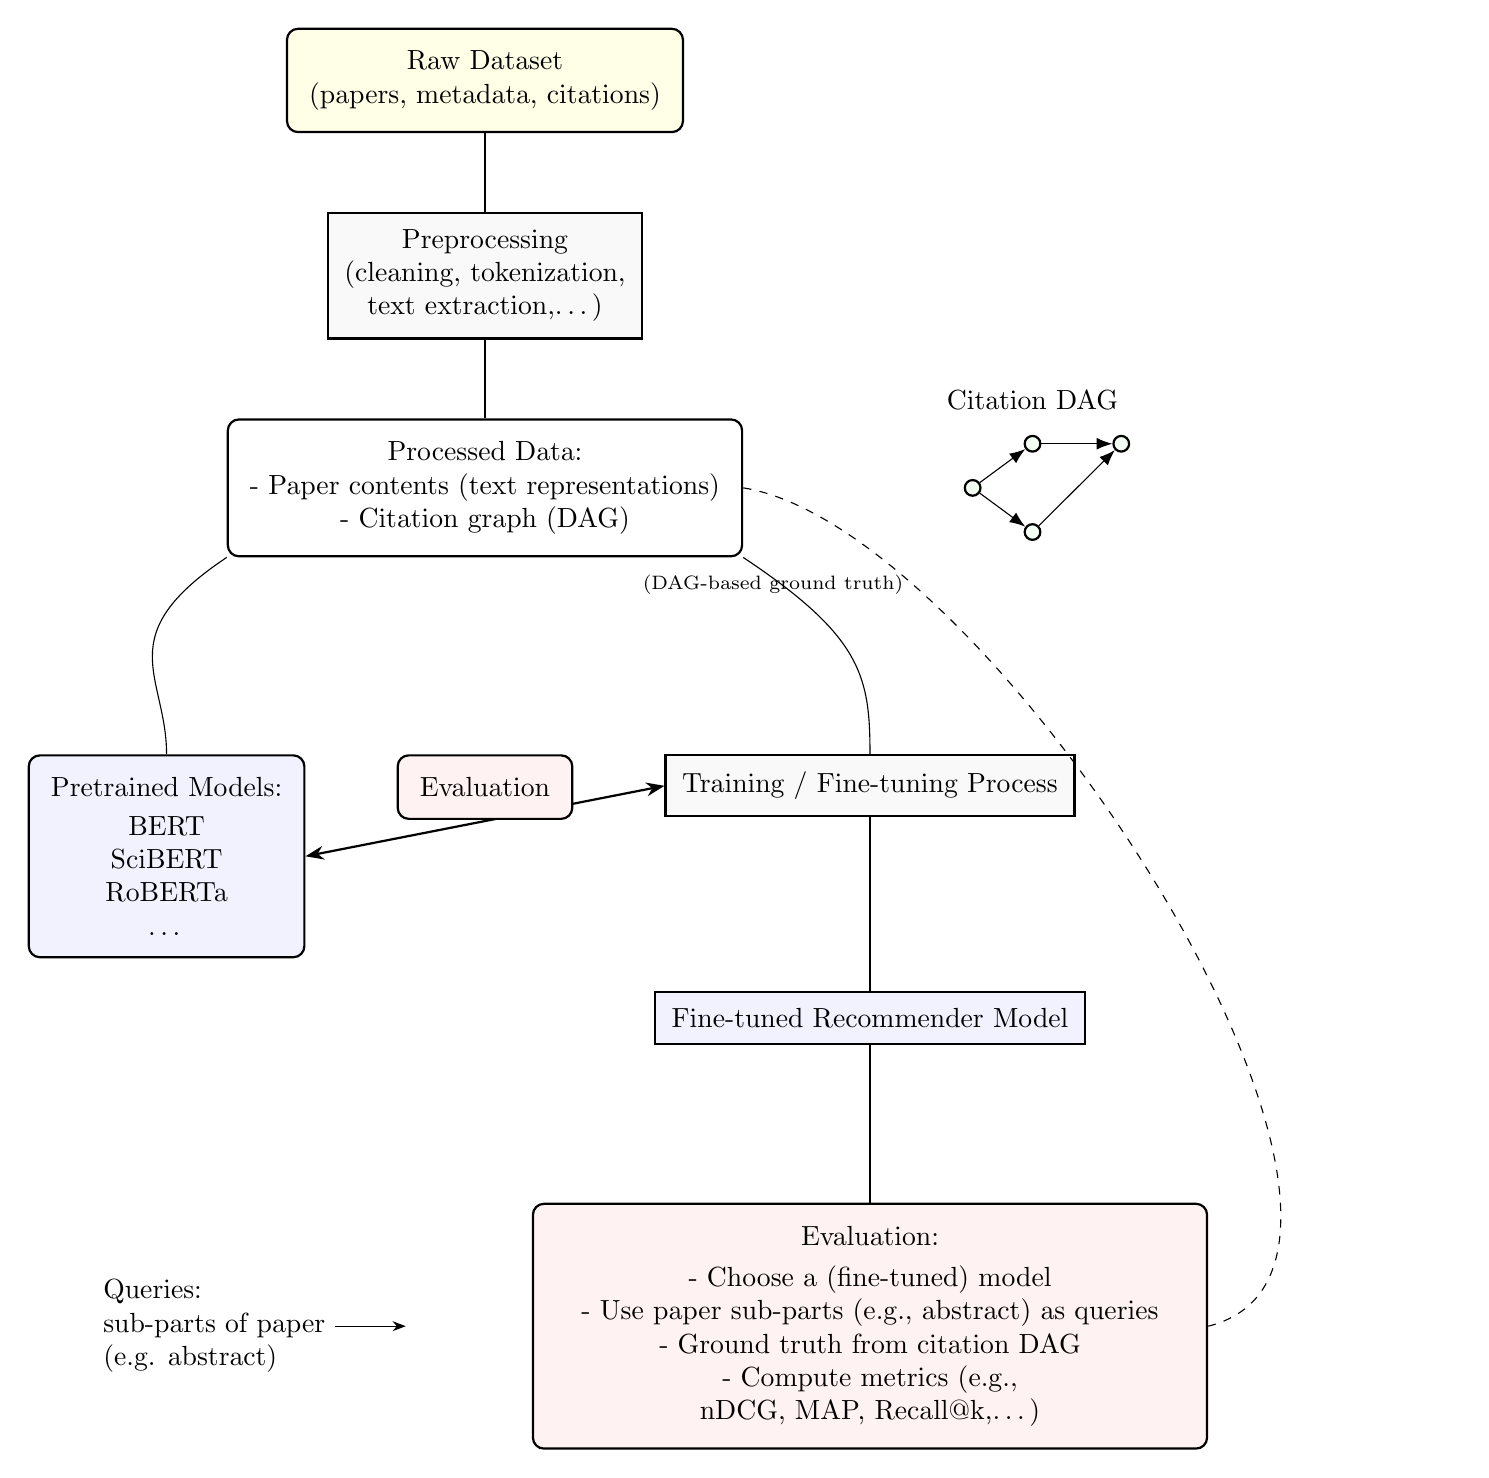
\begin{tikzpicture}[
    node distance=1cm and 1.5cm,
    >=Latex,
    >=Stealth,
    box/.style={rectangle, rounded corners, draw, thick, align=center, inner sep=8pt},
    process/.style={rectangle, draw, thick, align=center, inner sep=6pt, fill=gray!5},
    model/.style={rectangle, draw, thick, align=center, inner sep=6pt, fill=blue!5},
    dagnode/.style={circle, draw, thick, inner sep=2pt, fill=green!5},
    every edge/.style={draw, thick, -{Latex[length=3mm,width=2mm]}}
    ]

    % Top: Dataset input
    \node[box, fill=yellow!10] (dataset) {Raw Dataset\\(papers, metadata, citations)};

    % Preprocessing steps
    \node[process, below=of dataset] (preprocess) {Preprocessing\\(cleaning, tokenization,\\text extraction,\dots)};

    % Processed data: paper contents + DAG
    \node[box, below=of preprocess] (processed) {Processed Data:\\
      - Paper contents (text representations)\\
      - Citation graph (DAG)
    };

    % Small DAG sketch to the right of processed
    \node[dagnode, right=2.8cm of processed] (g1) {};
    \node[dagnode, above right=0.4cm and 0.6cm of g1] (g2) {};
    \node[dagnode, below right=0.4cm and 0.6cm of g1] (g3) {};
    \node[dagnode, right=0.9cm of g2] (g4) {};
    \draw[-{Latex[length=2mm]}] (g1) -- (g2);
    \draw[-{Latex[length=2mm]}] (g1) -- (g3);
    \draw[-{Latex[length=2mm]}] (g2) -- (g4);
    \draw[-{Latex[length=2mm]}] (g3) -- (g4);

    % Label for DAG
    \node[align=left, above=0.2cm of g2] (daglabel) {Citation DAG};

    % Pretrained models box
    \node[box, fill=blue!5, below left=2.5cm and -1.0cm of processed] (models) {Pretrained Models:\\[2pt]
      BERT\\
      SciBERT\\
      RoBERTa\\
      \dots
    };

    % Training process box
    \node[process, below right=2.5cm and -1.0cm of processed] (training) {Training / Fine-tuning Process};

    % Bidirectional arrows between models and training
    \draw[<->, thick] (models.east) -- node[above]{fine-tuning} (training.west);

    % Arrows from processed data to both models and training (features / supervision)
    \draw (processed.south west) .. controls +(-1.5,-1.0) and +(0,1.0) .. (models.north);
    \draw (processed.south east) .. controls +(1.5,-1.0) and +(0,1.0) .. (training.north);

    % Fine-tuned model
    \node[model, below=2.2cm of training] (finetuned) {Fine-tuned Recommender Model};

    \draw (training.south) -- (finetuned.north);

    % Evaluation block
    \node[box, fill=red!5, below=2.5cm of processed] (evaluation) {Evaluation};

    % Position evaluation roughly below fine-tuned and processed
    \node[box, fill=red!5, below=2.0cm of finetuned, text width=8cm] (evaldetail) {Evaluation:\\[3pt]
      - Choose a (fine-tuned) model\\
      - Use paper sub-parts (e.g., abstract) as queries\\
      - Ground truth from citation DAG\\
      - Compute metrics (e.g., nDCG, MAP, Recall@k,\dots)
    };

    % Arrows into evaluation
    \draw (finetuned.south) -- (evaldetail.north);
    \draw[dashed] (processed.east) .. controls +(3.2,-0.5) and +(3.2,0.8) .. (evaldetail.east);
    \node[below right=0.1cm and -1.4cm of processed] {\scriptsize (DAG-based ground truth)};

    % Arrow chain top-down
    \draw (dataset) -- (preprocess);
    \draw (preprocess) -- (processed);

    % Optional: label for query / ground truth split
    \node[align=left, left=2.5cm of evaldetail] (qlabel) {Queries:\\sub-parts of paper\\(e.g. abstract)};
    \draw[->] (qlabel.east) -- ++(0.9,0);

  \end{tikzpicture}
  \caption{Just a placeholder AI slop \color{red}TODO REPLACE}
  \label{fig:system-overview-dag}
\end{figure}

\newpage

\printbibliography[title=References]

\end{document}
